\documentclass[12pt, a4paper, titlepage]{article}
\usepackage{style}
\pagestyle{empty}


\begin{document}

\maketitle
\clearpage

\section{Kroneckerin kokonaisluvut}

Maagikko Kroneckerin mielestä ainoastaan kokonaisluvut ovat normaaleja lukuja. Kaikki muut luvut ovat hänen mielestään paholaisen aikaansaannosta.


Selvitä seuraavista yhtälöistä ne joiden ratkaisut mielyttäisivät Kroneckeriä.

\begin{equation}
2x^2-3=4
\end{equation}
\begin{equation}
x^3-x=0
\end{equation}
\begin{equation}
3a+3=5
\end{equation}
\begin{equation}
x^2-1=0
\end{equation}
\begin{equation}
\cos(x)=-1
\end{equation}
\begin{equation}
\frac{x}{3}=7
\end{equation}
\begin{equation}
-b+4=6
\end{equation}
\begin{equation}
\frac{3x^2-18x+24}{x-4}=0
\end{equation}
\begin{equation}
x^2+1=0
\end{equation}
\begin{equation}
-2x+6x^2=7
\end{equation}
\begin{equation}
\sqrt{x+2}=4
\end{equation}
\begin{equation}
\frac{x^2-4}{x-2}=0
\end{equation}
\begin{equation}
e^{ix}+1=0
\end{equation}

Vihje: Mikäli jokin yhtälöistä ei ratkea helposti, ei kannata huolestua. Joukosta saattaa löytyä kompia...

\begin{figure}[h]
    \centering
    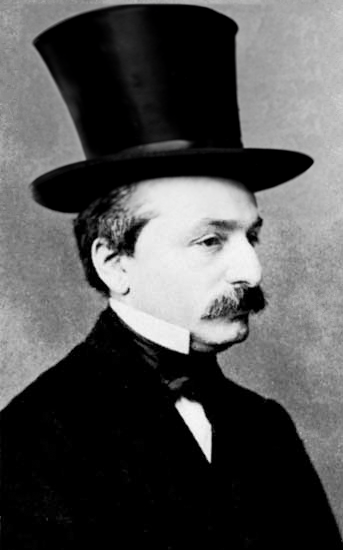
\includegraphics[width=0.15\textwidth]{kuvat/kronecker ja hattu.png}
    \caption*{Leopold Kronecker (1823-1891)}
\end{figure}

\input{tehtavat/cantorin_ympyrä}
\clearpage

\section{Pythagoran kolmio}

Peikko Pythagora työskentelee Draculan linnan työmaalla. Hänen tehtävänään on tukea rakennustelineet. Jotta telineistä tulisi tukevat, täytyy niiden kulmiin asentaa suorakulmaiset kolmiot. Pythagora on kuitenkin unohtanut suorakulmansa kotiin. Hän on mitannut $8 \text{cm}$, $15 \text{cm}$ ja $18 \text{cm}$ palat. Saako Pythagora näistä paloista rakennettua suorakulmaisen kolmion?

\begin{figure}[h]
    \begin{center}
    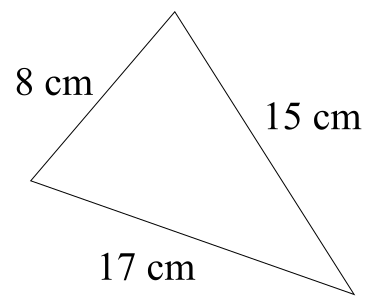
\includegraphics[width=0.5\linewidth]{kuvat/pythagoran_kolmio}
    \end{center}
\end{figure}
\clearpage

\section{Merirosvojen valuuttaongelma}

Merirosvot ovat tunnetusti petollisia henkilöitä. Tämä petollisuus aiheuttaa epäluuloa merirosvosatamissa. Kaupankäynti on satamissa vaikeata, koska myyjät pelkäävät, että ostaja yrittää tarjota heille väärennettyjä kolikoita. 


Tortugan satamassa toimii tämän takia kaksi kolikoita tutkivaa kultaseppää: Bolzanon ja Weierstrass. He osaavat tunnistaa väärennetyn kolikon aidosta. Ilmaiseksi kultasepät eivät kuitenkaan kolikoita tutkineet.


Bolzano veloittaa 20 dublonin perusmaksun, jonka lisäksi jokaisesta kilosta tarkastettavia kultakolikoita joutui pulittamaan yhden dublonin lisää.

Weierstrass puolestaan veloittaa 4 dublonin perusmaksun ja 5 dublonia per kilo tarkasteltavia kultakolikoita.

\begin{enumerate}
    \item Kumpaa kultaseppää kannattaa käyttää mikäli tarkastettavia kultakolikoita on 6 kg?
    \item Millä kultakolikkomäärällä kultasepät ovat yhtä edulliset?
    \item Paljonko kultakolikoita saa tarkastettua 34 dublonilla Bolzanon luona? Entäs Weierstrassin?
\end{enumerate}

\begin{figure}[h]
    \centering
    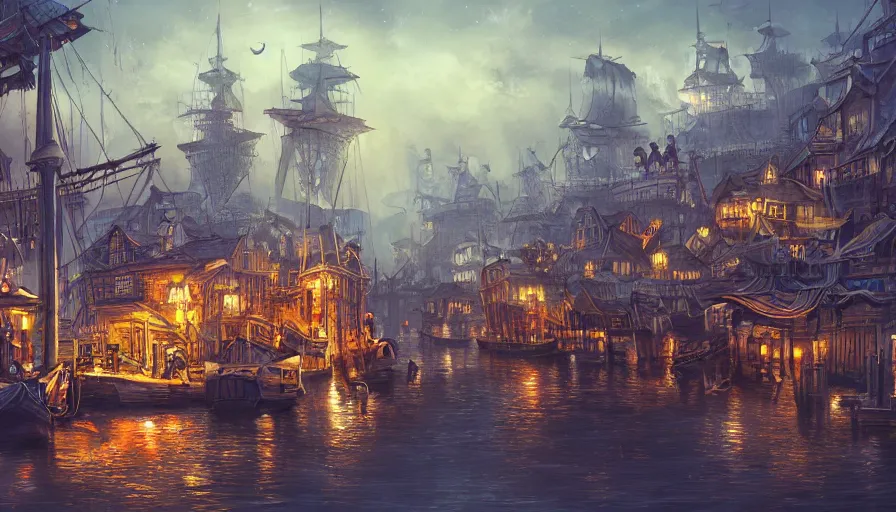
\includegraphics[width=0.75\linewidth]{kuvat/merirosvo_satama.png}
\end{figure}
\clearpage

\section{Eukliden suorakulmio}

Hirviö Euklides haluaa jakaa suorakulmion muotoisen kivenlohkareen kahteen täydellisesti saman kokoiseen palaan. Palat jakavan leikkaussuoran täytyy kulkea ulkopuolisen pisteen kautta. Euklidella on käytössä ainoastaan täysin suora keppi ja valkoinen liitu. Kuinka Euklides onnistuu?

\begin{figure}[h]
    \centering
    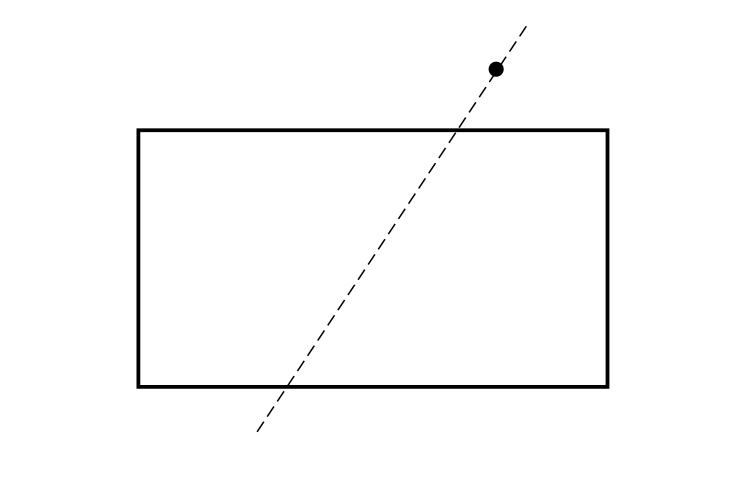
\includegraphics[width=0.6\linewidth]{kuvat/suorakulmio_kahteen_osaan.png}  
\end{figure}
\clearpage

\section{Descartes ja kaksinkertainen kulma}

Piru Descartes löytää yöllisen retkensä aikana maahan piirretyn terävän kulman. Descartes kärsii ahdistuneisuushäiriöistä eikä kulma mielytä häntä. Hän haluaisi että kulma on tasan kaksinkertainen alkuperäiseen nähden. Hänellä on kuitenkin mukanaan ainoastaan suora keppi, harppi ja punainen liitu. Kuinka Descartes saa muutettua kulman haluamallaan tavalla?

\begin{figure}[h]
    \centering
    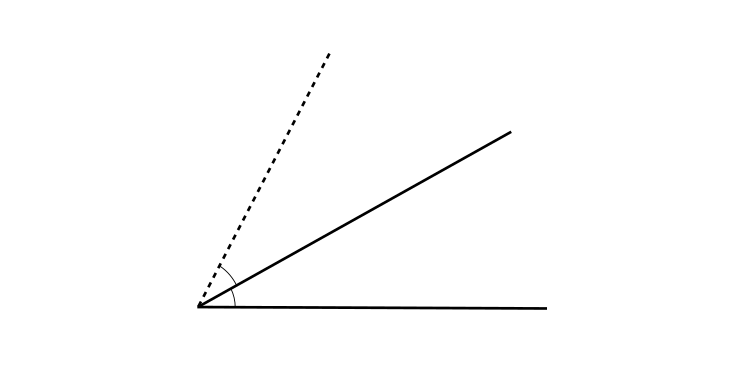
\includegraphics[width=0.7\linewidth]{kuvat/uusi_kulma.png}
\end{figure}
\clearpage

\section{Krampin ostosreissu}

Matematiikkamörkö Kramp kulki aavekaupungin läpi. Hän näki erään liikkeen näyteikkunassa seuraavan tekstin

\begin{equation*}
    \sqrt{-1} \quad 2^3 \quad \sum \quad \pi
\end{equation*}

Näky herautti veden Krampin kielelle ja hän päätti pistäytyä liikkeessä. Missä liikkeessä Krampi vieraili?

Vihje: $i^2=-1$


Puolen tunnin kuluttua Kramp jatkoi eteenpäin autiolla ostoskadulla. Seuraavan näyteikkunan kohdalla hän pelästyi pahan päiväisesti. Mitä Kramp näki näyteikkunassa?

Vihje: Vastaus on noin $7{,}71053\cdot10^{1976}$
\clearpage

\section{Gaussin rohtokauppa}

Kummitus Gauss pitää Kyöpelinvuorella rohtokauppaa. Kaupassa myydään rohtoja ja liemiä niitä tarvitseville noidille. Gauss valmistaa erittäin myrkyllistä \textit{venenum} -liuosta alla olevan reseptin mukaan. Resepti on erittäin vanha ja siitä on jäljellä enää taulukko, jossa kerrotaan myrkkyjauheen määrä eri tilavuuksissa. 

Eräänä päivänä Gaussin kauppaan saapui huolestunut asiakas, joka halusi tietää myrkkyliuoksen pitoisuuden. Gauss on kuitenkin hukannut reseptistä sen sivun, jolla liuoksen pitoisuus kerrotaan. Osaatko auttaa Gaussia?

\begin{table}[h]
  \centering
    \begin{tabular}{| c | c |}
    \hline
    Liuoksen lopputilavuus (ml) & Myrkkyjauheen määrä (mg) \\
    \hline
    60 & 23{,}3 \\
    80 & 35{,}6 \\
    100 & 40{,}1 \\
    120 & 52{,}7 \\
    140 & 56{,}3 \\
    160 & 64{,}9 \\
    180 & 79{,}9 \\
    200 & 87{,}5 \\
    220 & 88{,}2 \\
    \hline
    \end{tabular}
  \caption*{Ohjeet \textit{venenum} -liuoksen valmistukseen}
\end{table}

Eräs asiakas tulee kysymään Gaussilta saisiko myrkkyliuosta $500 \text{ml}$ annoksen. Gauss lupaa toimittaa asiakkaalle kysytyn annoksen. Paljonko Gauss tarvitsee annokseen myrkkyjauhetta? 


Lisätehtävä: Miksi Kyöpelinvuoren kylässä asuva fyysikkofenrir Maxwell kritisoi Gaussin lupausta suuresta annoksesta? 
\clearpage

\section{Fermat’n kasino}

Vampyyri Fermat järjestää kartanossaan iltaisin uhkapeli-iltoja. Yksi pelaajista, kreivi Pascal, on kovasti tykästynyt rulettiin. Pascal uskoo, että pelaajat jäävät siinä keskimäärin voitolle.


Jokaisen peli-illan jälkeen Pascal lähtee kuitenkin tyhjin taskuin kotiin. 


Selittääkö epäonni Pascalin huonon menestyksen peli-illoissa?


Fermat’n rulettipöydässä yksi veikkaus maksaa 1 €.


\begin{figure}[h]
    \begin{center}
    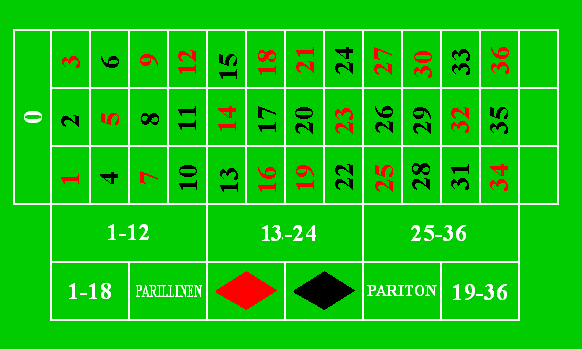
\includegraphics[width=0.8\linewidth]{kuvat/ruletti.png}
    \caption*{Rulettipöytä}
    \end{center}
\end{figure}

\begin{table}[h]
  \centering
    \begin{tabular}{| l | l | l |}
    \hline
    Panostusvaihtoehto & Selite & Voitto \\
    \hline
    Yksi numero & Pelimerkki sijoitettu yhdelle numerolle & 36 € \\
    Kaksi numeroa & Pelimerkki sijoitettu 2:n numeron rajalle & 18 € \\
    Neljä numeroa & Pelimerkki sijoitettu 4:n numeron kulmaan & 9 € \\
    \hline
    Tusinat & 1-12, 13-24 tai 25-36 & 3 € \\
    Väri & musta tai punainen & 2 € \\
    Pienet/isot & 1-18 tai 19-36 & 2 € \\
    Parillinen/pariton & & 2 € \\
    \hline
    \end{tabular}
  \caption*{Ruletin voitonjako}
\end{table}

Vihje: Mitä odotusarvo kertoo?
\clearpage

\section{Valehtelevat kummitukset}

Kummitusten kylässä asuu kolme viisasta kummitusta: Boole, Tarski ja Gödel. He ovat koko elämänsä etsineet todistusta nimeltä ''kaiken teoria''. Kaikki kummituksista eivät kuitenkaan ole todistusta vielä löytäneet. Kummitukset eivät kuitenkaan halua paljastaa tätä, joten mikäli he eivät ole löytäneet todistusta, valehetelevat he. Mikäli kummitus on löytänyt todistuksen, puhuu hän totta. 

\begin{figure}[h]
    \begin{center}
    
\includegraphics[width=0.5\linewidth]{kuvat/kolme_kummitusta.jpg}
    \end{center}
\end{figure}

Pääset haastattelemaan jokaista kummitusta. He kaikki ovat niukkasanaisia ja suostuvat kertomaan pelkästään seuraavaa:

Boole: ''Tarski ei ole löytänyt todistusta tai Gödel ei ole löytänyt todistusta.''

Tarski: ''Minä olen löytänyt todistuksen ja Boole ei ole löytänyt todistusta.''

Gödel: ''Tarski ei ole löytänyt todistusta.''


Kuka/ketkä kummituksista ovat löytäneet todistuksen?

\clearpage

\section{Riemannin ikkuna}

\begin{wrapfigure}{r}{0.4\textwidth}
  \begin{center}
    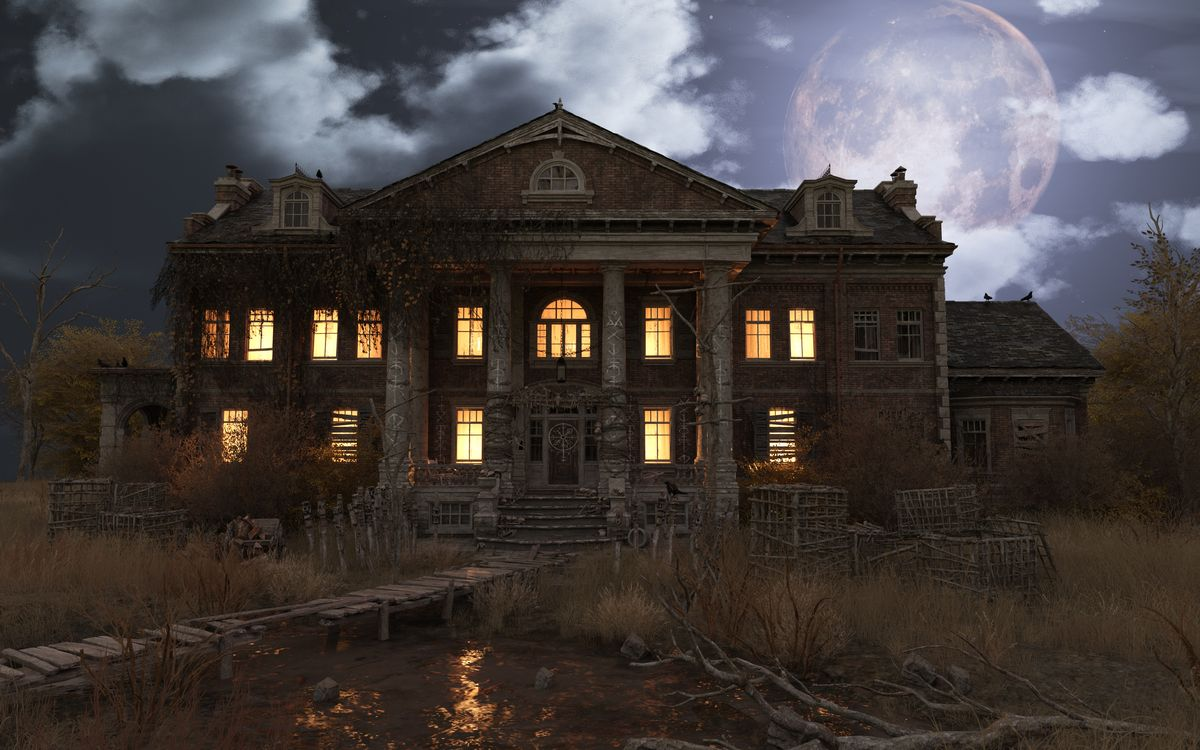
\includegraphics[width=0.38\textwidth]{kuvat/riemann_kartano.jpg}
  \end{center}
\end{wrapfigure}

Luuranko Riemann on rakentamassa itselleen suurta ja pelottavaa kartanoa. Hän haluaa kartanon julkisivulle näyttävän ikkunan. Riemann päättää tehdän ikkunasta parabelin muotoisen. Ikkunan korkeudeksi tulee $2 \ \text{m}$ ja leveydeksi $4 \ \text{m}$.


Paljonko Riemann tarvitsee lasia ikkunan valmistamiseen?

Lisätehtävä: Paljonko puuta ikkunan kehyksiin tarvitaan?
\clearpage

\section{Gabrielin viinipikari}

\begin{wrapfigure}{r}{0.25\textwidth}
    \begin{center}
    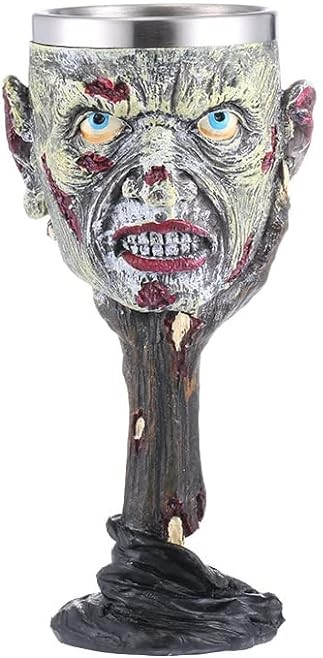
\includegraphics[width=0.23\textwidth]{kuvat/viinipikari_hirvio.jpg}
    \caption*{Vanhat pikarit}
    \medskip
    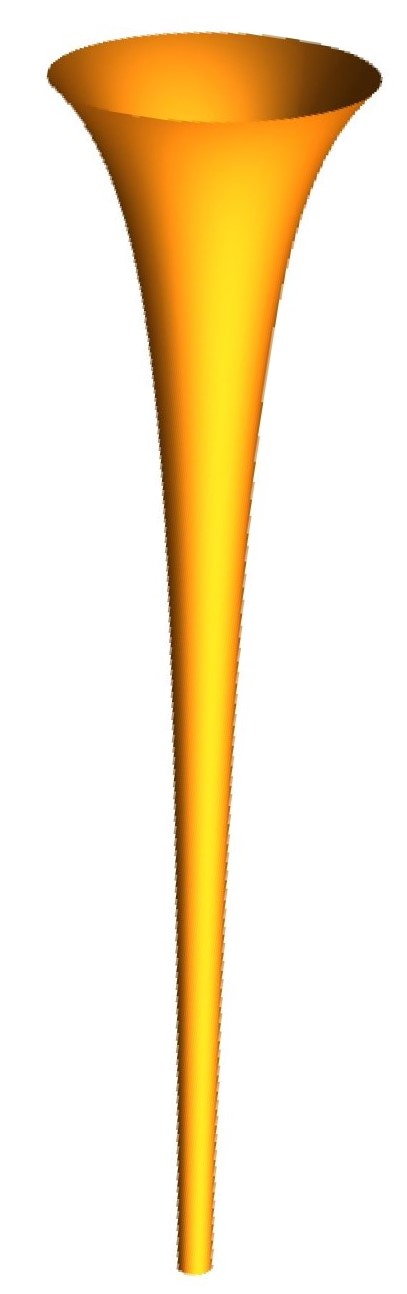
\includegraphics[width=0.23\textwidth]{kuvat/gabrielin_torvi.jpeg}
    \caption*{Torricellin idea uudeksi pikariksi}
    \end{center}
\end{wrapfigure}

Titanit Gabriel ja Torricelli istuivat titaanien baarissa tulivuori Vesuviuksen juurella. Gabriel ei pitänyt baarin viinipikareista. Ne olivat hänen mielestään liian epämääräisen muotoiset. Hän ei myöskään pitänyt pikarien väristä. Gabriel halusi pikarin, joka on päällystetty kultaisella maalilla ja on geometrisen muotoinen.

Torricelli ehdotti Gabrielille pikaria, joka on muodostettu käyrän $\frac{1}{x}$ pyörähdyspinnan osasta $x \ge 1$.

\begin{enumerate}
\item Pystyykö pikarin ulkopuolen maalaamaan realistisesti kultaisella maalilla?
\item Pystyykö pikarin täyttämään viinillä piripintaan?
\end{enumerate}

Vihje 1: Laske paljonko viiniä ja maalia tarvittaisiin.


Vihje 2: Pyörähdyskappaleen pinta-alalle ja tilavuudelle löytyy kaavat MAOLista.
\clearpage

\section{Taylorin laskinpulma}

\begin{wrapfigure}{r}{0.3\textwidth}
    \begin{center}
    
\includegraphics[width=0.28\textwidth]{kuvat/taylor_monsteri.jpg}
    \end{center}
\end{wrapfigure}

Monsteri Taylorilla on hirveiden, kauheiden ja karmivien esineiden sekatavarakauppa. Taylorilla on kuitenkin ongelma, koska hänen superlaskimensa on mennyt rikki. Kaupan nurkasta löytyi onneksi vanha ja pölyinen laskukone. Laskukoneella pystyy kuitenkin tarkastelemaan pelkästään polynomiyhtälöitä. 

\begin{enumerate}
\item Taylorin täytyisi laskea taajusgeneraattorin ominaisuuksia. Ongelmana on kuitenkin se, että generaattori muodostaa funktion $f(x) = \cos(x)$ muotoista vaihtovirtaa. Pystytkö auttamaan Tayloria ja muodostamaan polynomifunktion, joka approksimoi funktiota $f(x) = \cos(x)$ pisteen $x = 0$ ympäristössä?

\item Taylorin pitäisi myös laskea eksponentiaalisesti lisääntyvien myrkkykärpästen määrä. Pystytkö auttamaan Tayloria ja muodostamaan polynomifunktion, joka approksimoi funktiota $g(x) = e^x$ pisteen $x = 0$ ympäristössä?
\end{enumerate}

Vihje 1: Polynomifunktio on muotoa $a_nx^n+\ldots+a_2x^2+a_1x+a_0$

Vihje 2: Polynomifunktiota kannattaa lähteä rakentamaan vakiotermistä $a_0$. Tämän jälkeen ensimmäisen asteen termille pitäisi saada \textbf{kulmakerroin} $a_1$.


Vihje 3: Mitäköhän Taylorin sarja mahtaa tehdä?

\end{document}
